% !TeX root = ../article-enso.tex

\section{Response of the epipelagic community to extreme \nino{} events}
\label{sec:nino-epi}

This section focuses on describing the simulated size-dependent response of the epipelagic community to ENSO and understanding the mechanisms responsible for this response. Here, we will specifically study the epipelagic community response to the three strongest \nino{} events over the historical period, namely those of 1982/83, 1997/98 and 2015/16 \citep{santosoDefiningCharacteristicsENSO2017}. During these events, the central and eastern Pacific has warmed by more than 2°C (Figure \ref{fig:nemo-had-sst}a), moving the warm waters and associated atmospheric convection from the west to the central and eastern Pacific. The atmospheric signature of these \nino{} has had dramatic climatic consequences, including droughts and forest fires in countries bordering the western Pacific, but also torrential rains and floods along the south American coast \citep{caiClimateImpactsNino2020}. Their oceanic signature also had major impacts on marine ecosystems and biodiversity, leading to significant disruptions in marine life and seabird populations \citep{valleImpact198219831987}, promoting large-scale marine heatwaves \citep{holbrookKeepingPaceMarine2020} and coral bleaching \citep{claarGlobalPatternsImpacts2018}.  The ocean response during each of these three extreme events has been extensively described and analyzed in terms of physics (e.g. \citealp{philanderChapter33Simulation1985, lengaigneOceanResponseMarch2002, puyModulationEquatorialPacific2019}), biogeochemistry (e.g. \citealp{barberBiologicalConsequencesNino1983, chavezBiologicalChemicalResponse1999, strammaObservedNinoConditions2016}) and marine ecosystems \citep{glynnNINOSOUTHERNOSCILLATION198219831988, glynnCoralBleachingMortality2001, eakin20142017Globalscale2019}. 

To isolate the generic response of epipelagic organisms to extreme \nino{} events, independent of the intrinsic characteristics of each event, we perform a composite analysis of these three extreme events, averaging monthly anomalies of temperature, ocean velocity, low trophic level  (LTL, i.e. phyto and zooplankton, particulate organanic matter) concentrations and biomass of the epipelagic community over the 1982-1983, 1997-1998 and 2015-2016 periods. These extreme \nino{} events are also followed by \nina{} conditions the following year (more intense in the case of the 1997/98 event), which also allows for a discussion  of the epipelagic community response mechanisms to \nina{} events. Although the temporal evolution and amplitude of the processes discussed below vary slightly between events, the relative importance of the processes discussed in our composite analysis remains qualitatively similar when these three extreme events are analyzed individually (not shown). 

\subsection{Model response from physics to ecosystems}

As major environmental drivers of the epipelagic biomass variability, Figure \ref{fig:hov_nemo_ape}a-c first depicts the temporal evolution of monthly equatorial anomalies in upper ocean temperatures, LTL concentration and zonal currents during and after extreme \nino{} events, in the form of equatorial time-longitude diagrams, with the January month preceding the onset of the \nino{} event as origin of time. The warming signal associated with \nino{} initiates in the central equatorial Pacific in early spring, then spreads rapidly to the eastern Pacific, intensifies during the summer and fall, peaks at the end of the calendar year, and finally  declines rapidly and transitions to \nina{} conditions the following spring (from April-y1, Figure \ref{fig:hov_nemo_ape}a). The development phase of \nino{} is also characterized by strong eastward surface currents anomalies in the western and central Pacific (Figure \ref{fig:hov_nemo_ape}b) induced by anomalous westerly winds, promoting warming of the central Pacific and eastward movement of the warm-pool toward the eastern equatorial Pacific. These current anomalies reverse at the peak of \nino{} and during \nina{}. The simulated plankton concentration anomalies largely mirror those of temperature, with a sharp decrease during \nino{} and an increase during \nina{} (Figure \ref{fig:hov_nemo_ape}.c). 

\begin{figure}[h!tp]
	\centering
	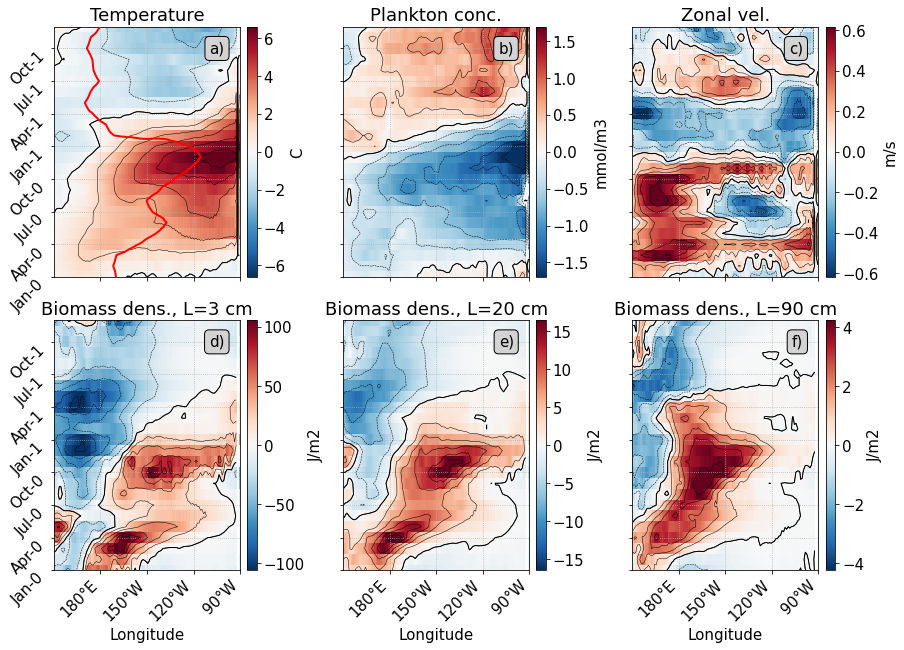
\includegraphics[scale=0.4]{plot_all_hovmoller_phys_oope.png}	
	\caption{Time-longitude diagrams in the equatorial Pacific of surface temperatures (in °C) (a), zonal velocity (in m/s) (b), low-trophic level concentrations (in mmol/m3) (c) and fish biomass anomalies (in J/m2) associated with extreme \nino{} events composite (3cm, 20cm and 90 cm in d, e, f, respectively). The eastern location of the warm pool (28\degree{} isotherm) is shown in red in (a).}	
	\label{fig:hov_nemo_ape}
\end{figure}

A similar analysis is then performed for epipelagic biomass for the three selected size classes (Figure \ref{fig:hov_nemo_ape}def). Their responses to \nino{} share common characteristics: positive biomass anomalies appear near the dateline early in the calendar year and propagate eastward toward the central Pacific until late spring (May/June-y0). These positive biomass anomalies in the central Pacific re-intensify in fall and then rapidly disappear in winter. They are also accompanied by a decrease in biomass in the western Pacific from the beginning of the \nino{} year. These negative anomalies persist after the \nino{} peak and during the subsequent \nina{} event but remain largely confined to the western Pacific. Despite similar behaviour, however, the response of the three size classes show some significant differences, including a westward shift in response as size class increases.

Figure \ref{fig:profiles} shows how these surface ENSO-related signals propagate in depth by providing climatological equatorial profiles of temperatures, zonal velocities, low-trophic level concentrations and epipelagic daytime biomass for the three size classes, as well as their boreal winter anomalies for extreme \nino{} composites. The climatological temperature profile indicates that the thermocline is deep in the western Pacific and shallow in the east, and flattens during \nino{}, resulting in warming in the east and cooling in the west (Figure  \ref{fig:profiles}a). The Equatorial Undercurrent also weakens strongly during \nino{}, while strong positive (i.e. eastward) current anomalies occur near the surface (Figure  \ref{fig:profiles}b). Low trophic level biomass, which is maximal in the upper 50m of the eastern Pacific, decrease during \nino{}, due to the flattening of the thermocline, which reduces the nutrient supply in the surface layers (Figure \ref{fig:profiles}c). Regarding the vertical extent of the epipelagic community, the climatological biomass for the three classes in the western Pacific extends from the surface to $100m$ in the western Pacific and decreases during \nino{} events. However, this decrease is not homogeneous along the vertical, with strong positive anomalies appearing around 40m in the west for intermediate and large sizes (Figure \ref{fig:profiles}def). These are induced by a narrowing of the vertical habitat, due to the shallowing of the thermocline. 
%The climatological biomass decrease rapidly towards the central Pacific to become negligible in the eastern part of the basin. This structure is significantly altered during extreme \nino{} events, where fish biomass increases from the surface to $100m$ depth in the central and eastern Pacific, with a maximum located near $40m$.

\begin{figure}[h!tp]
	\centering
	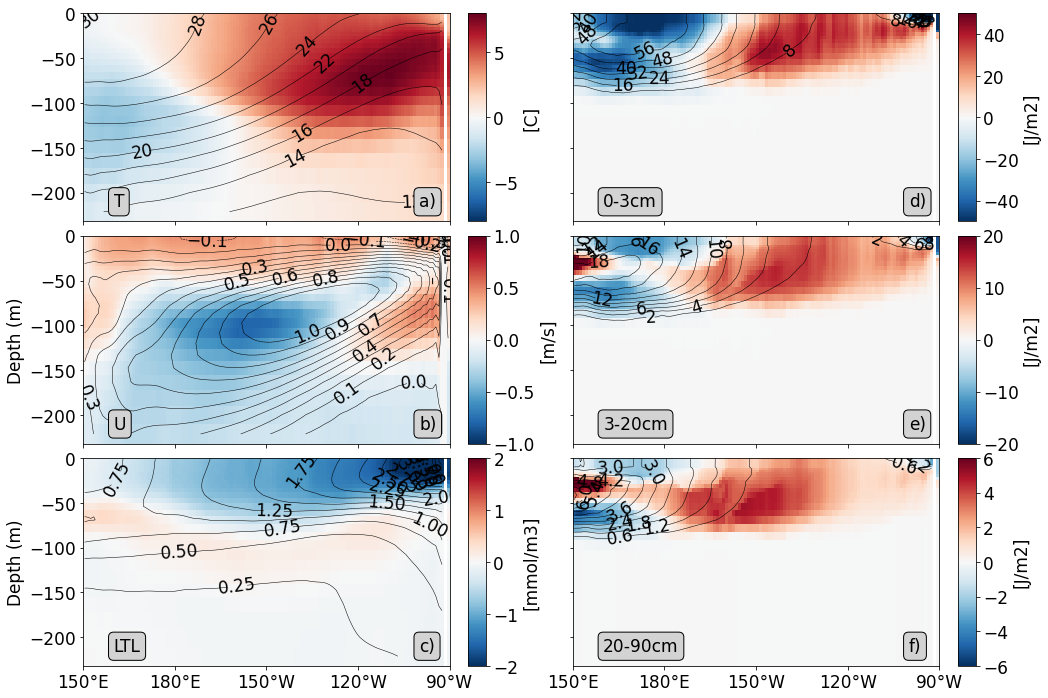
\includegraphics[scale=0.4]{figs/forage_mean_ond97.png}	
	\caption{Pacific equatorial profiles of temperature (a), zonal velocity (b), low-trophic level concentration (c) and fish biomass (d for small, e for intermediate and f for large sizes). Mean values are represented as black contour lines and \nino{} anomalies are represented in colors.}	
	\label{fig:profiles}
\end{figure}

\subsection{Processes driving the epipelagic upper-ocean response}

The contribution of the different processes responsible for the epipelagic response to \nino{} (Figure \ref{fig:hov_nemo_ape}def) is now assessed by performing the same equatorial time-longitude diagrams for the main tendency terms (right members of equation \ref{eq:apecosm_trend}) and their temporal integral, which represents their contribution to the total biomass change (as done in \citealt{guietMovementShapesStructure2022} to seperate passive advection and active swimming). We also analyze key parameters of the biological response to changing environmental conditions, namely growth rate ($\gamma$ in equation \ref{eq:apecosm_trend}), functional response (equation \ref{eq:repfonct}) and predation mortality rates ($M$ in equation \ref{eq:apecosm_trend}). Because the relative importance of these processes varies among size classes, these analyses are discussed separately for each size class.

Figure \ref{fig:fig7} provides a synthesis of the respective contributions of biological (i.e. the combined action of growth and predation) and physical (i.e. the combined action of advection and diffusion) processes on the epipelagic biomass response to ENSO for each of the three size classes. A first result is that the relative importance of biological processes decreases as fish size increases for two reasons. First, predation is size-based in the APECOSM model, resulting in high predation pressure on small organisms, which decreases with size since larger organisms have fewer predators in the model. Second, growth includes a flux term and a source term (see equation \ref{eq:apecosm_trend}) that are both dependent on temperature. The source term controls biomass production and varies as ${\gamma}/{w}$, which scales linearly with $w^{-\frac{1}{3}}$ and thus decreases strongly with size.

The decrease of the small and intermediate size biomass in the western Pacific is thus primarily the result of biological processes. In the central and eastern Pacific, the combined action of dynamic and biological processes accounts for the increase in biomass during \nino{} (Figure \ref{fig:fig7}a-f) while these processes largely offset each other when the equatorial Pacific reverses to \nina{} conditions, resulting in small  changes in biomass in this region. For the largest size class, physical processes (Figure \ref{fig:fig7}i) explain most of the biomass changes (Figure \ref{fig:fig7}g), with biological processes being negligible (Figure \ref{fig:fig7}h).

The action of dynamic processes on biomass evolution is simple. It results from the transport of biomass from the western to the central Pacific in response to the strong eastward currents anomalies that occur during extreme \nino{} conditions. It is experienced in a similar way by all size organisms, since the ocean current anomalies during \nino{} (up to $0.6 m.s^{-1}$, see Figure \ref{fig:hov_nemo_ape}c) dominate the active velocity anomalies by a factor of $\approx\ 1000$ for small sizes, $20$ for intermediate sizes and $3$ for large sizes (not shown). 

\begin{figure}[h!tp]
	\centering
	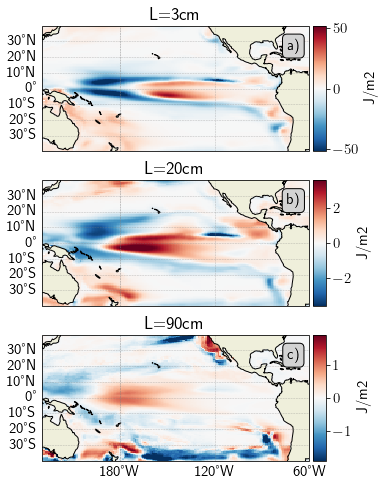
\includegraphics[scale=0.4]{figs/fig7.png}	
	\caption{Time-longitude diagrams in the equatorial Pacific of total (left), biologically (middle, predation plus growth terms) and dynamicly (right, advection plus diffusion) induced interannual variations in fish biomass (in $J.m^{-2}$) associated with extreme \nino{} events composites for small (top), intermediate (middle) and large (bottom) sizes.}
	\label{fig:fig7}
\end{figure}

The significant and sometimes dominant contribution of biological processes for small and medium size classes, however, is more difficult to understand intuitively because it results from the combined action of predation mortality and growth. Therefore, we further detail the respective contribution of predation and growth and their driving factors for small and medium size classes on Figure \ref{fig:fig8} and Figure \ref{fig:fig9} respectively.

For small size classes (3cm), the effects of predation mortality balance the effects of growth (Figure \ref{fig:fig8}bc), resulting in a net effect of biological processes that is much smaller than the effect of each biological process considered in isolation (Figure \ref{fig:fig8}a). Growth leads to an increase in biomass at the onset of \nino{} in the central Pacific (between dateline and 150\degree{}W), that spreads eastward to its peak. These positive biomass anomalies then decrease slightly during the following \nina{} conditions (Figure \ref{fig:fig8}b).

Figure \ref{fig:fig8}e shows the functional response, which controls the predation swimming speed (that is proportional to the functional response's gradient), the vertical distribution and swarming level of epipelagic fish, which in turn control their availability to predators.  Despite its importance in controlling growth and reproduction, our analysis indicates that the decrease in functional response is not the primary driver of biomass changes, since negative functional response anomalies are associated with positive biomass anomalies.

Instead, the increase in growth rate east of the dateline during \nino{} closely follows the evolution of the anomalous warming (Figure \ref{fig:fig8}e), suggesting that changes in growth rate are largely driven by the influence of temperature on fish physiology. In contrast to the central and eastern Pacific, the growth rate decreases in the western Pacific as it cools from July of the \nino{} year, contributing to a decrease in biomass. Although these growth rate negative anomalies in the western Pacific are smaller than the positive ones in the eastern part, their impact on the biomass, which is proportional to the biomass itself (cf. equation \ref{eq:apecosm_trend}) is greater since biomass levels are ten times larger in the west than in the east (see black contours in Figure \ref{fig:mean_ond97_ape}).

As mentioned previously, predation-induced changes in biomass are largely opposite to growth-induced changes  (Figure \ref{fig:fig8}bc). Predation-induced changes decrease biomass in the central and eastern Pacific and increase biomass in the far western Pacific (Figure \ref{fig:fig8}c), closely following the changes in biomass of intermediate size predators (Figure \ref{fig:fig8}f). Despite their opposite effect on biomass, growth effects generally slightly dominate those of predation, explaining most of the decrease in small size classes in the western Pacific during \nino{} and the subsequent \nina{}, and reinforcing the biomass increase in the central Pacific induced by dynamic processes during \nino{}. An exception is the very early decrease in biomass simulated near the dateline from February of the \nino{} year, which is not driven by growth rate changes (Figure \ref{fig:fig8}b) but rather by increased predation by intermediate size organisms at the \nino{} onset (Figure 8c,f).

\begin{figure}[h!tp]
	\centering
	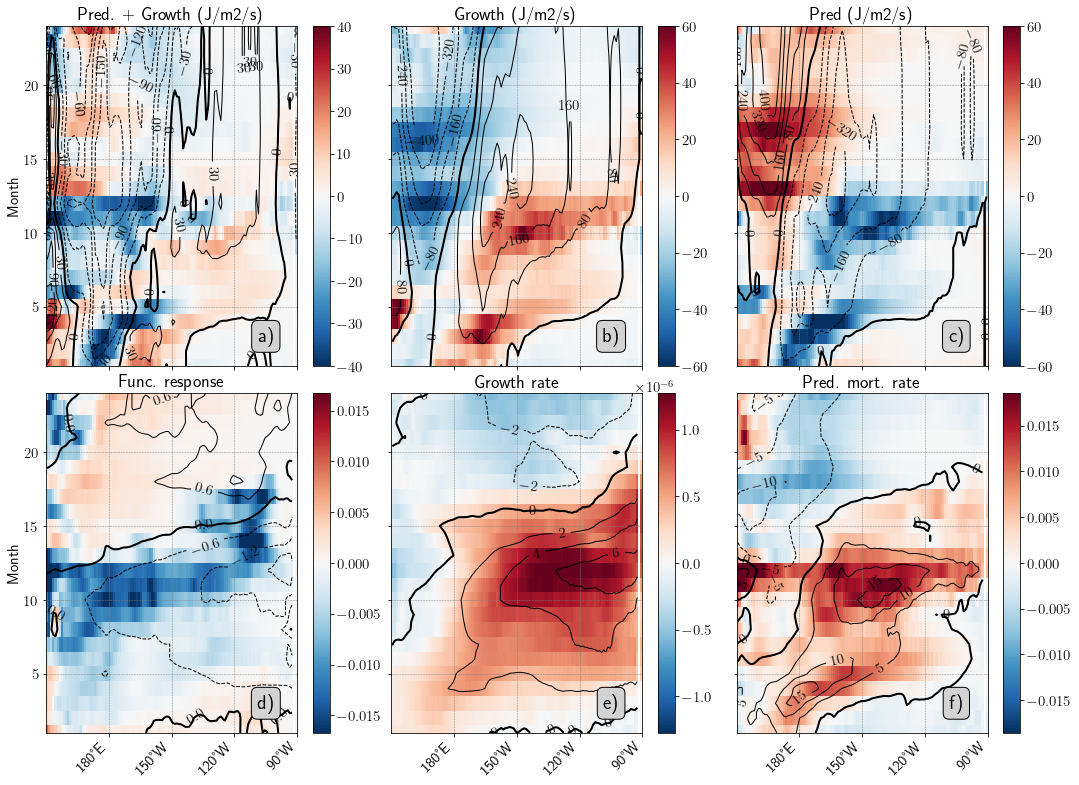
\includegraphics[scale=0.4]{figs/fig8.png}	
	\caption{Time-longitude diagrams in the equatorial Pacific of interannual anomalies of small sizes biomass trends ($J.m^{-2}.s^{-1}$; in colors) and time-integrated trends ($J.m^{-2}$; in contours) associated with extreme \nino{} events composite for predation plus growth (a), growth (b) and predation (c). Same as (a-c) but for interannual anomalies of the functional response (no unit; in colors) and planktonic prey biomass density ($mmol.m^{-3}$; in contours) (d), growth rate ($kg.day^{-1}$; in colors) and temperature (°C; in contours) (e) and predation mortality rate ($day^{-1}$; in colors) and intermediate size biomass ($J.m^{-2}$; in contour) (f).}
	\label{fig:fig8}
\end{figure}

% ---------------- to complete
The growth and predation induced biomass changes for the intermediate size classes are similar to those simulated for small size classes (Figure \ref{fig:fig9}): they are opposite and of the same order of magnitude, with growth effects generally dominating predation effects. Growth increases fish biomass in the central Pacific from the onset to the peak of \nino{}. However, the influence of temperature on fish physiology is no longer the dominant factor of biologically induced biomass changes for intermediate size organisms as it was for small organisms. In contrast to small size classes, changes in growth rate largely reflect changes in functional response, which is increasing in the central Pacific due to both warmer waters (increased swimming speed controlling the attack rate parameter in the functional response) and increased food availability (due to the increased biomass of small organisms), both of which contribute to increase the biomass of intermediate size organisms in the central Pacific. In the western Pacific, the growth rate decreases only very modestly (Figure \ref{fig:fig9}b) but, as seen for small size classes, this translates into a large reduction of growth-induced biomass from October onwards since its effect is proportional to biomass, which is ten times larger in the western than in the eastern Pacific (Figure \ref{fig:mean_ond97_ape}).
On the other hand, predation generally mitigates the effects of growth, reducing biomass in the central Pacific through increased predation by large size classes there and increasing biomass in the western Pacific during the subsequent \nina{} through reduced predation. This evolution largely resembles those obtained for small sizes, albeit with a modest westward shift. The changes induced by the combination of these two processes are generally dominated by growth, except in the western Pacific during \nino{} development where the  decrease in biomass from February onwards is due to increased predation by large organisms. As for small sizes, the decrease in biomass in the western Pacific during \nino{} and the subsequent \nina{} are initially due to increased predation followed by a reduction in growth, while dynamicrocesses dominate the biomass increase east of the dateline with a smaller contribution from growth.

\begin{figure}[h!tp]
	\centering
	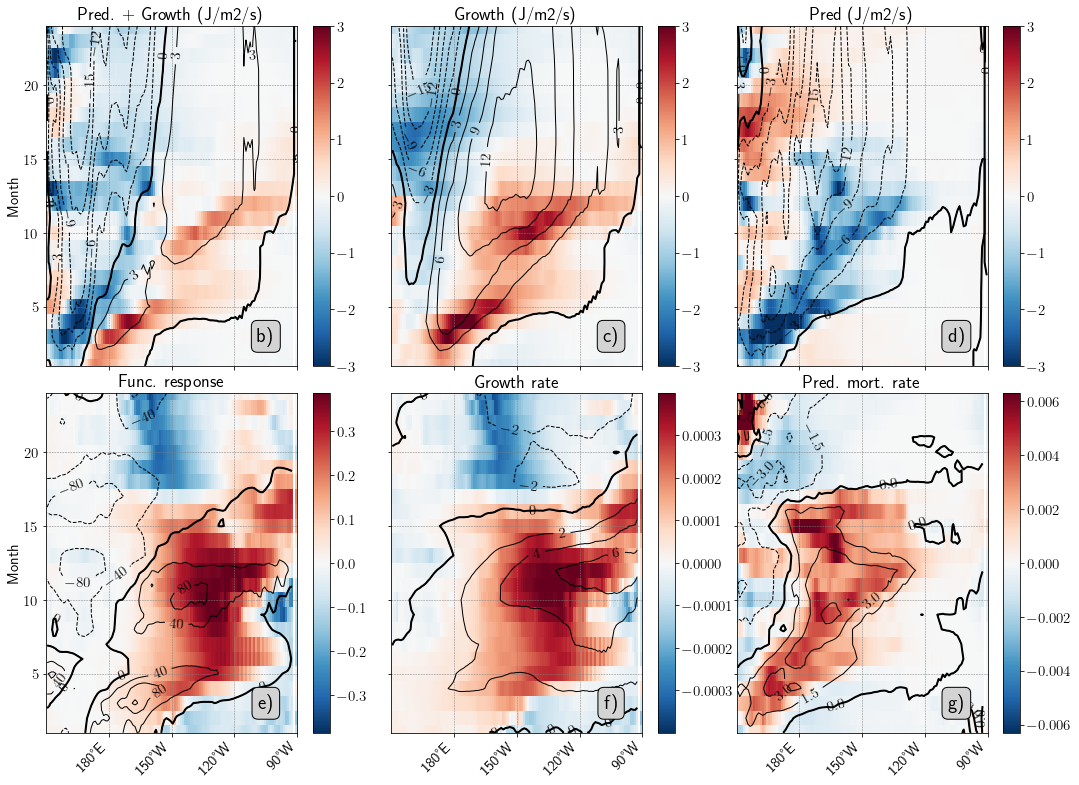
\includegraphics[scale=0.4]{figs/fig9.png}	
	\caption{Time-longitude diagrams in the equatorial Pacific of interannual anomalies of intermediate sizes biomass trends ($J.m^{-2}.s^{-1}$; in colors) and time-integrated trends ($J.m^{-2}$; in contours) associated with extreme \nino{} events composite for predation plus growth (a), growth (b) and predation (c). Same as (a-c) but for interannual anomalies of the functional response (no unit; in colors) and small prey biomass density ($J.m^{-2}$; in contours) (d), growth rate ($kg.day^{-1}$; in colors) and temperature (°C; in contours) (e) and predation mortality rate ($day^{-1}$; in colors) and large size biomass ($J.m^{-2}$; in contour) (f).}
	\label{fig:fig9}
\end{figure}

Figure \ref{fig:proc_summary} provides a brief summary of the different processes involved in the epipelagic response to interannual ENSO variability that has been discussed in this section.

\begin{figure}[h!tp]
	\centering
        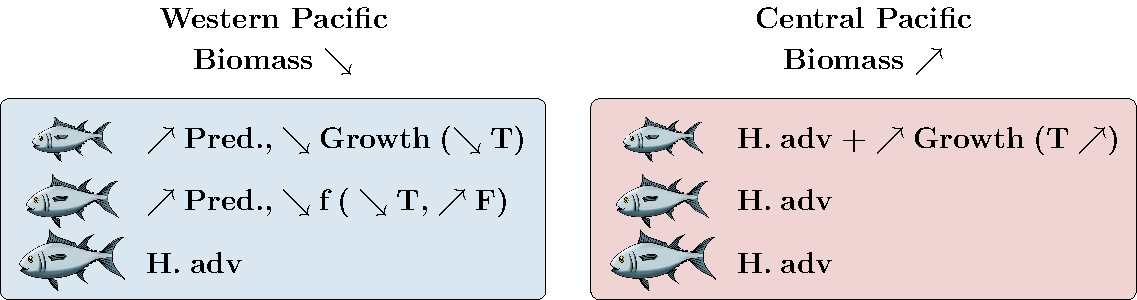
\includegraphics[scale=0.6]{figs/conclusion/conlusion_fig.pdf}	
        \caption{Summary of the processes involved in the response of epipelagic biomass to \nino{} conditions.  $Pred.$ is predation, $T$ is temperature, $A+D$ is advection/diffusion, $f$ is the functional response and $F$ is food concentration.}
	\label{fig:proc_summary}
\end{figure}



\subsection{Generalization}

All the analyses presented above focused on the equatorial Pacific, where ENSO physical and biogeochemical signatures are the strongest. To ascertain the response of off equatorial regions to ENSO,  Figure \ref{fig:mean_ond97_ape} further provides maps of climatological epipelagic biomass for the three size classes as well as their boreal winter anomalies for extreme \nino{} composites.  In average, epipelagic fish biomass is largest both sides of the equator and in the equatorial western Pacific (Figure \ref{fig:mean_ond97_ape}abc), while smaller biomasses  are found in the eastern Pacific. In agreement with the equatorial analyses provided on Figure \ref{fig:hov_nemo_ape}, Figure \ref{fig:mean_ond97_ape}a indicates that during \nino{}, small epipelagic fish biomass increases in the equatorial eastern Pacific and decreases in the western Pacific. In addition, Figure \ref{fig:mean_ond97_ape}a reveals that this biomass also decreases both sides of the equator, further highlighting that the biomass does not only shift eastward during \nino{} but also equatorward.
As size increases, positive anomalies associated with \nino{} conditions expand westward and poleward while negative anomalies weaken and expand equatorward. 

\begin{figure}[h!tp]
	\centering
	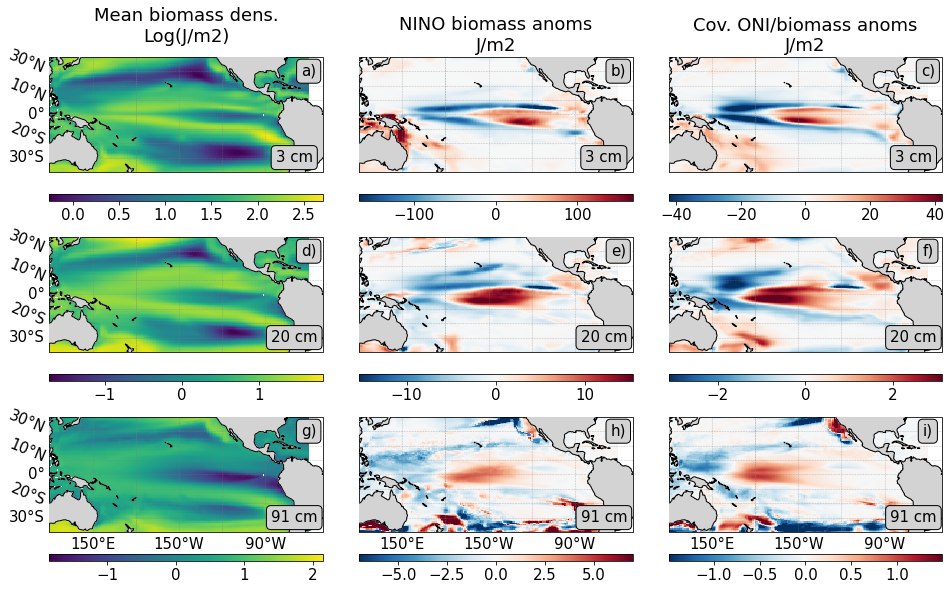
\includegraphics[scale=0.4]{figs/map_mean_anom_OND_97.png}	
	\caption{Maps of boreal winter (DJF) biomass anomalies for extreme \nino{} events composites (left column) and covariance of fish biomass anomalies with the ONI index (right column) for small (upper line), intermediate (middle line) and large sizes (lower line). Black contours correspond to the climatological biomass density distribution (log-scale).}	
	\label{fig:mean_ond97_ape}
\end{figure}


To insure that the biomass response described for extreme \nino{} events is representative of ENSO variability in general, Figure \ref{fig:mean_ond97_ape}def shows the covariance maps computed between the monthly ONI index and the detrended fish biomass anomalies for the three size classes over the 1958-2018 period. This analysis reveals that the patterns in extreme \nino{} composites are very similar to covariance analyses, although amplitudes are about four times larger for extreme events. This  difference  in amplitude is related to the fact that the covariance analysis also includes weaker \nino{} events (such as the 1986, 1991, 1994, 2002, 2004 and 2009 events) as well as \nina{} events, which are known to have weaker physical and biogeochemical signatures. Nevertheless, the very good match between the covariance maps and the extreme \nino{} composites indicates that the biomass response and related mechanisms discussed above for the three major \nino{} events are also representative of other ENSO events.
